\documentclass{article}

\usepackage{graphicx, caption}
\usepackage{float}

\title{Random Facts About Me}
\date{2023-09-16}
\author{Gloria Lee} 

\begin{document}
  \pagenumbering{gobble}
  \maketitle
  \newpage
  \pagenumbering{arabic}

  \begin{abstract}
    \noindent Hello! This document was made with the purpose for me to practice using LaTeX and complete my CS190 assignment, while my hopes for you, the reader, is to learn some random facts about me. 
    I hope you enjoy what's to come... 
  \end{abstract}

  \section{Basic Information}
  \textbf{My full name is Gloria Goeun Lee.}
    \paragraph{Paragraph}
    A fun fact about my name is that I actually named myself 'Gloria' after the hippo in Madagascar \cite{MOVIE:1}. My family immigrated to the US when I was five, and my parents gave my sisters 
    and I the option to choose our 'English' names. Madagascar was my favorite movie at that time, and Gloria was my favorite character. So, that's why I'm Gloria!
    \subparagraph{Subparagraph}
    My middle name Goeun is my Korean name. I was named by my grandfather. My two older sisters and I all share the '-eun' syllable in our names. Figure \ref{fig:sisters} shows me and my sisters, Esther (Chaeeun) and Sunny (Sieun), with my mom.

    \hspace{1cm}
    
    \begin{figure}[hbt!]
      \begin{center}
      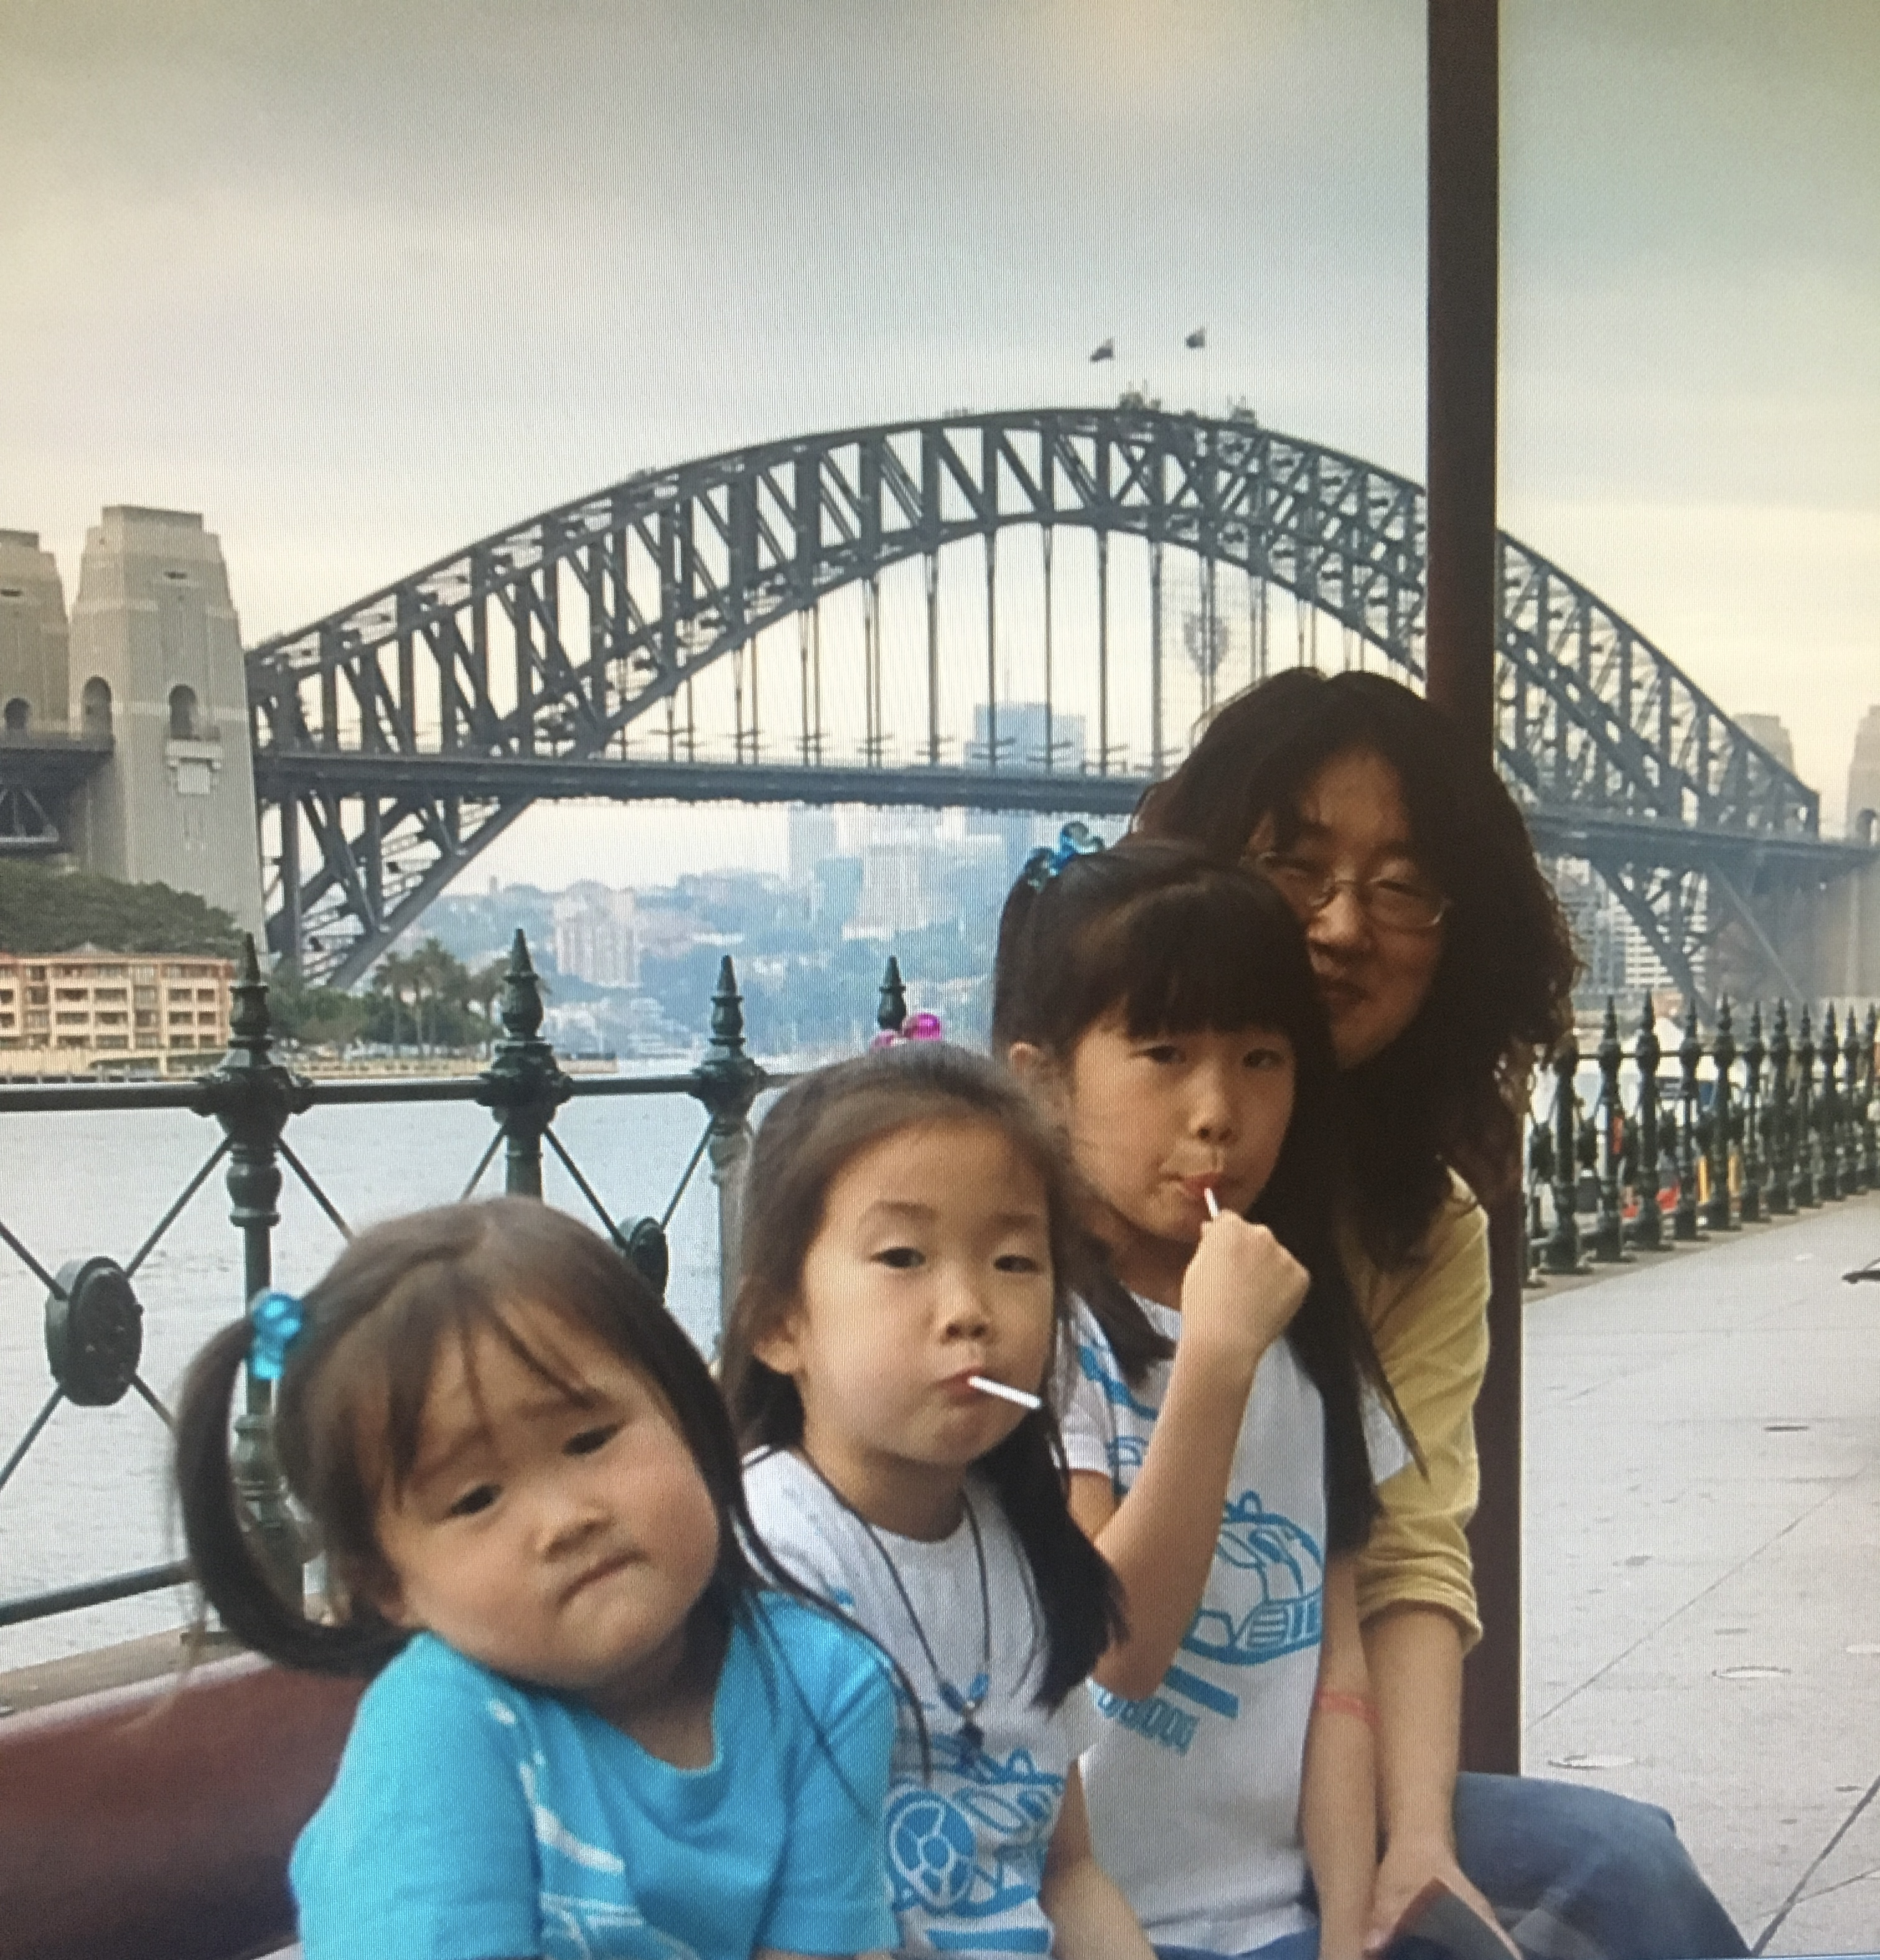
\includegraphics[width=2in]{little sisters and me.jpg}
      \captionsetup{justification=centering}
      \caption{My mom, sisters, and I sitting on a bench. \\Me wondering why I don't have a lolipop.}
      \label{fig:sisters}
      \end{center}
    \end{figure}

  \noindent \textbf{I am from the Greater Seattle Area.}

    \paragraph{Paragraph}
    My hometown is Mukilteo, WA. It's a 40-minute drive north of Seattle, but I just say I am from Seattle. I love taking advantage of the beautiful nature in Washington, 
    so I try to go hiking and camping often with my friends when I am home. Figure \ref{fig:mountain} shows a view from one of my favorite nature places. 

    \begin{figure}[hbt!]
      \begin{center}
      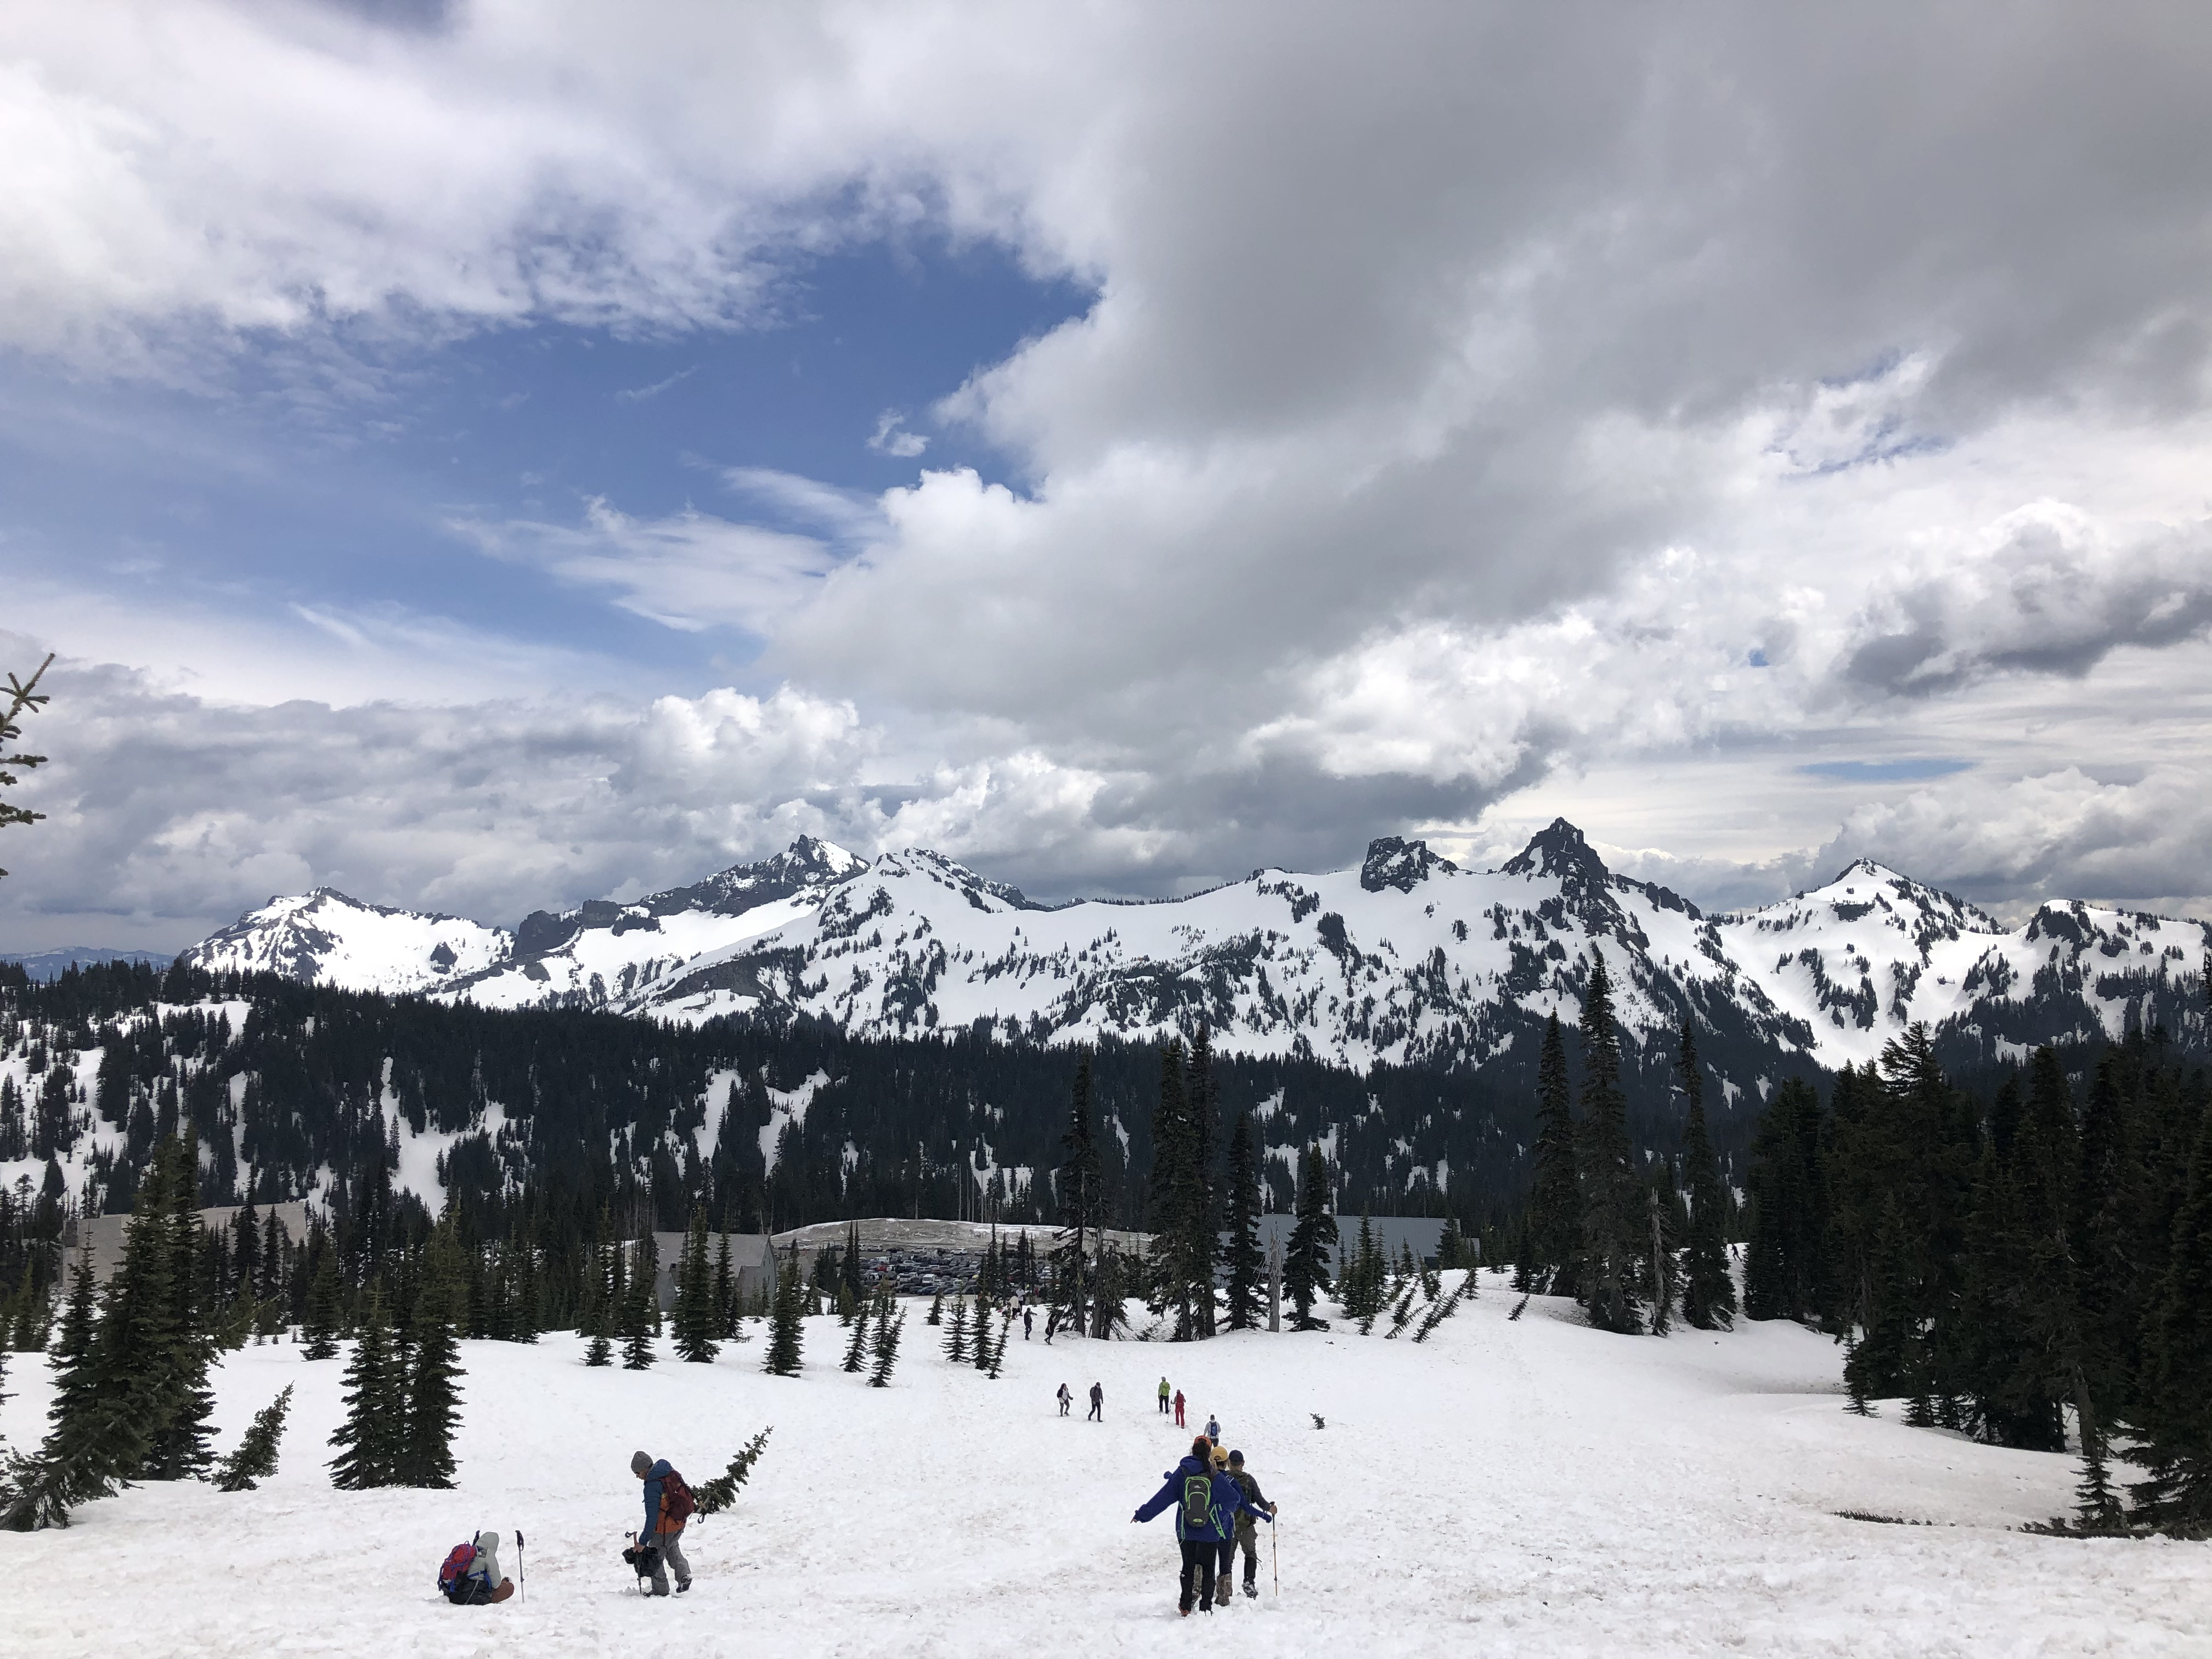
\includegraphics[width=3in]{mtRainier-1.jpg}
      \captionsetup{justification=centering}
      \caption{A trail on Mount Rainier with so much snow!}
      \label{fig:mountain}
      \end{center}
    \end{figure} 


  \section{Favorite Things}
  In my free time, I like to watch Korean dramas/shows, casually play basketball, and go on slow, long runs. 
  I don't read for leisure often, but when I do, I tend to read memoirs. Here (Ref \ref*{listOfBooks}) is a list of some of my favorite books. 

    \begin{itemize}
      \label{listOfBooks}
      \item "Know My Name" by Chanel Miller \cite{BOOK:1},
      \item  "1984" by George Orwell \cite{BOOK:2},
      \item "Crying in H Mart" by Michelle Zauner \cite{BOOK:3}
    \end{itemize}

  \hspace{1cm}

  \noindent I do listen to music often, especially when I study, so I tend to like softer sounds. I am a big Bruno Major fan! 
  Table \ref{tab:music} lists my top 3 artists and songs from them. 

    \begin{table}[ht!]
      \begin{center}
        \caption{My favorite artists} 
        \label{tab:music} 
        \begin{tabular}{c|c|c} 
          \textbf{ranking} & \textbf{name} & \textbf{fav song}\\
          \hline
          1 & Bruno Major & "Nothing" \cite{SONG:1} \\
          2 & Lizzy McAlpine & "ceilings" \cite{SONG:2} \\
          3 & Lake Street Dive & "Hypotheticals" \cite{SONG:3} \\
        \end{tabular}
      \end{center}
    \end{table}


  \bibliographystyle{plain}
  \bibliography{autobiography} 

\end{document}